
\subsection{Event Builder}
The Event Builder collects information from all upstream services, correlates information from subdetectors into particles, performs a general particle identification scheme, and organizes the resulting information into a standardized data bank structure.

First, one charged particle is assigned to each reconstructed track.  Associated calorimeter, scintillator, and C{e}renkov detector responses are then assigned to that particle based on geometric (and eventually timing) coincidence between the response and track, with matching criteria corresponding to the given detector.  Then, a similar procedure is followed for creating neutrals particles, except seeding is with unassociated ECAL and CND responses instead of tracks.

Then, a start time is assigned to the entire event, which serves as our single, most precise reference time on which all time-based particle identification relies.  This is based on the optimal charged particle candidate, which is the highest energy lepton or hadron with precise timing information.  A correction is then performed using the RF signal from the accelerator, combined with the event vertex position, effectively aligning the event start time to our best measure of bunch-crossing time at the primary interaction in the target.

A basic particle identification scheme is then performed.  For charged particles, first calorimetry and Cerenkov information is used to positively identify electron and positron candidates.  Remaining charged particles are then assumed to be hadrons and assigned based solely on timing information.  An identification quality factor is assigned based on the relevant detector responses and their resolutions.  For neutral particles, identity assignment is only made for neutrons and photons, based only on timing and topological information.

The resulting information is organized into standardized output bank structures for physics analyis, see \ref{sec:dsts}.  This includes particle four-vectors, all their associated detector responses, and global event information such as beam RF and helicity information.

\subsubsection{Particle Identification Performance}

\begin{table}[htpb]
  \begin{center}
    \label{tab:pidmatrix}
    \begin{tabular}{|c|cccccc|}\hline
          & \multicolumn{6}{|c|}{Truth}\\        
          & $e$ & $\pi$ & $K$ & $p$ & $n$ & $\gamma$ \\\hline
  $e$     &     &       &     &     &     &          \\ 
  $\pi$   &     &       &     &     &     &          \\ 
  $K$     &     &       &     &     &     &          \\ 
  $p$     &     &       &     &     &     &          \\ 
  $n$     &     &       &     &     &     &          \\ 
 $\gamma$ &     &       &     &     &     &          \\\hline 
    \end{tabular}
  \caption{Pariticle identification matrix, based on simulation for particles between 1 and 4 GeV momentum.  The diagonal elements are correctly identified, while the off-diagonal elements are misidentified.}
  \end{center}
\end{table}

\vspace{1in}
\begin{figure}
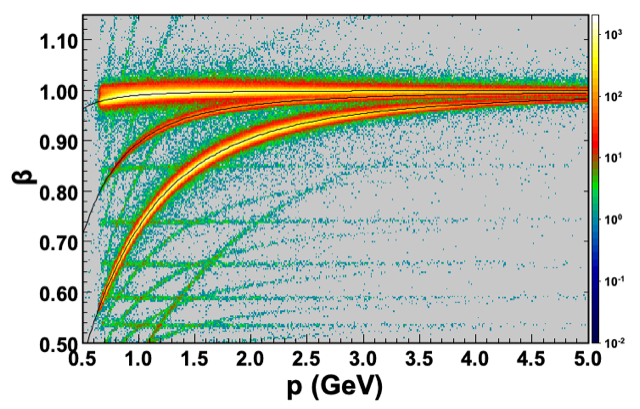
\includegraphics[width=0.45\textwidth]{pics/betavsp1.png}
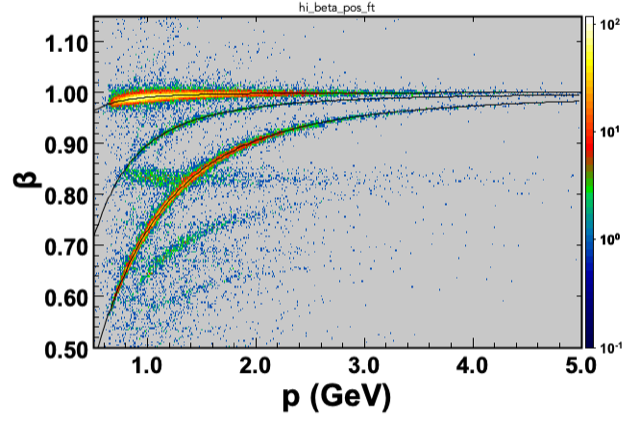
\includegraphics[width=0.45\textwidth]{pics/betavsp2.png}
\caption{Beta versus p for events with an electron in the FD (left plot) and in the FT (right plot).
}
\label{fig:betavsp}
\end{figure}

\begin{figure}
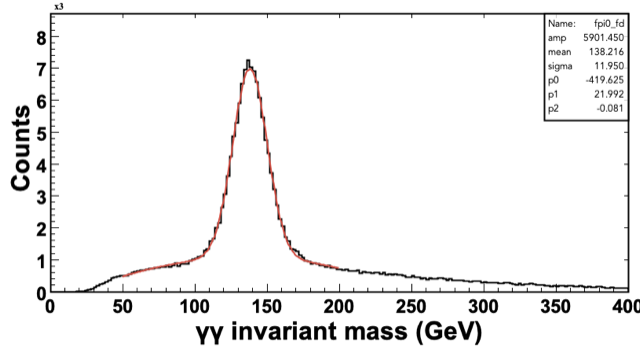
\includegraphics[width=0.45\textwidth]{pics/pi0mass.png}
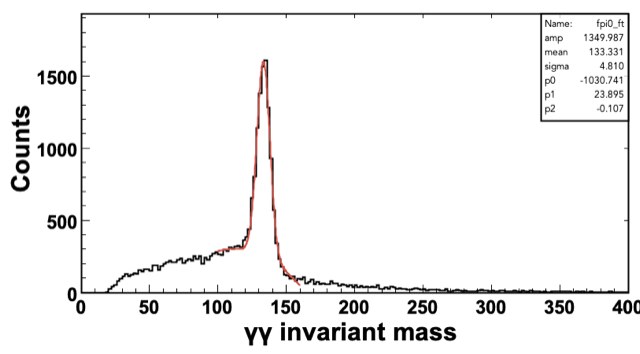
\includegraphics[width=0.45\textwidth]{pics/pi0mass2.png}
\caption{Reconstructed $\pi^{0}\rightarrow \gamma \gamma$ candidates using EC (left plot) and FT (right plot) information.
}
\label{fig:pi0mass}
\end{figure}

